% Figure: biased sparse inference-time sampling.
%
% Geometry (in figure units; treat as proxies for microns):
%   axon A trunk:  (0.5, 5) -- (10, 5)
%   axon A branch: (3.5, 5) -- (5.7, 7)        (branch point at (3.5, 5))
%   axon B trunk:  flat at y=2 from x=0.5..5, bezier bump up to (7, 4.4),
%                  bezier back down to (9, 2), flat to (10, 2)
%   r_branch = 1.4   (drawn around the branch point)
%   r_prox   = 1.3   (drawn around the A trunk node nearest to B's peak)
%
% A node is colored ("interesting") iff it falls within r_branch graph-
% distance of a branch node OR within r_prox Euclidean distance of a node
% in a different connected component. Otherwise it is grey ("skipped").
%
% Membership has been precomputed by hand; see comments next to each
% \foreach loop for the math.

\documentclass[border=10pt,tikz]{standalone}
\usepackage{tikz}
\usepackage{amsmath}
\usepackage{xcolor}
\usetikzlibrary{positioning, calc, arrows.meta, backgrounds, shapes.geometric}

% --- Palette ---
\definecolor{compA}{HTML}{C0392B}    % red    -- axon A
\definecolor{compB}{HTML}{2471A3}    % blue   -- axon B
\definecolor{branchR}{HTML}{D68910}  % amber  -- r_branch
\definecolor{proxR}{HTML}{6C3483}    % purple -- r_prox
\definecolor{idle}{HTML}{B0B7BD}     % grey   -- skipped

\begin{document}
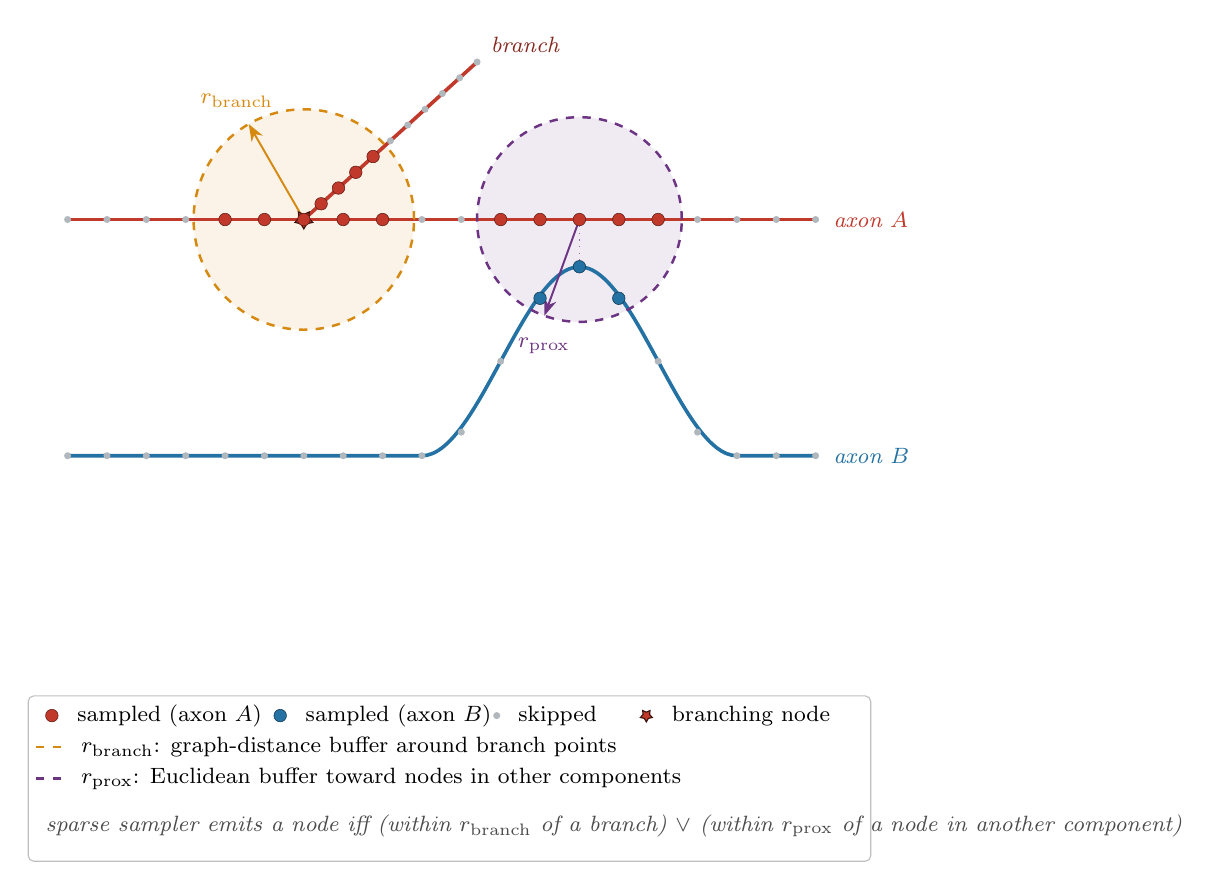
\begin{tikzpicture}[
    >=Stealth,
    font=\small,
    skelA/.style    ={line width=1.3pt, color=compA, line cap=round},
    skelB/.style    ={line width=1.3pt, color=compB, line cap=round},
    rBranch/.style  ={dashed, line width=0.9pt, color=branchR},
    rProx/.style    ={dashed, line width=0.9pt, color=proxR},
    intA/.style     ={circle, fill=compA, draw=compA!50!black,
                      line width=0.2pt, inner sep=1.6pt},
    intB/.style     ={circle, fill=compB, draw=compB!50!black,
                      line width=0.2pt, inner sep=1.6pt},
    skipped/.style  ={circle, fill=idle, inner sep=0.9pt},
    branchMark/.style={star, star points=5, star point ratio=0.55,
                       fill=compA, draw=compA!30!black, line width=0.4pt,
                       inner sep=2.4pt},
]

% ====================================================================
% Background shading of the two radius regions (drawn before everything)
% ====================================================================
\begin{scope}[on background layer]
    \fill[branchR!10] (3.5, 5) circle [radius=1.4];
    \fill[proxR!10]   (7.0, 5) circle [radius=1.3];
\end{scope}

% ====================================================================
% Axon A skeleton: trunk + branch
% ====================================================================
\draw[skelA] (0.5, 5) -- (10.0, 5);
\draw[skelA] (3.5, 5) -- (5.7, 7.0);

% ====================================================================
% Axon B skeleton: flat, bezier bump up to (7, 4.4), bezier back down
% ====================================================================
\draw[skelB]
    (0.5, 2.0) -- (5.0, 2.0)
    .. controls (5.7, 2.0) and (6.3, 4.4) .. (7.0, 4.4)
    .. controls (7.7, 4.4) and (8.3, 2.0) .. (9.0, 2.0)
    -- (10.0, 2.0);

% ====================================================================
% Radii outlines
% ====================================================================
\draw[rBranch] (3.5, 5) circle [radius=1.4];
\draw[rProx]   (7.0, 5) circle [radius=1.3];

% ====================================================================
% Radius annotations
% ====================================================================
% r_branch: arrow pointing upper-left from branch point to circle edge
\draw[branchR, line width=0.7pt, ->]
    (3.5, 5) -- ({3.5 + 1.4*cos(120)}, {5 + 1.4*sin(120)});
\node[color=branchR, anchor=south, font=\footnotesize] at (2.65, 6.30)
    {$r_{\mathrm{branch}}$};

% r_prox: arrow pointing lower-left from A node to circle edge
\draw[proxR, line width=0.7pt, ->]
    (7.0, 5) -- ({7.0 + 1.3*cos(-110)}, {5 + 1.3*sin(-110)});
\node[color=proxR, anchor=north, font=\footnotesize] at (6.55, 3.62)
    {$r_{\mathrm{prox}}$};

% Inter-axon distance illustration: thin segment between the closest
% pair of nodes from different components
\draw[proxR!70, line width=0.4pt, dotted] (7.0, 5) -- (7.0, 4.4);

% ====================================================================
% Branching node marker (drawn on top of the trunk)
% ====================================================================
\node[branchMark] at (3.5, 5) {};

% ====================================================================
% Axon labels on the right
% ====================================================================
\node[color=compA, anchor=west, font=\footnotesize\itshape] at (10.1, 5)
    {axon $A$};
\node[color=compB, anchor=west, font=\footnotesize\itshape] at (10.1, 2)
    {axon $B$};
\node[color=compA!70!black, anchor=south west, font=\footnotesize\itshape]
    at (5.75, 7.0) {branch};

% ====================================================================
% Skeleton nodes
% ====================================================================
% --- A trunk (x = 0.5..10.0 step 0.5) -------------------------------
% Interesting iff (a) within r_branch=1.4 of (3.5, 5) along trunk:
%   |x - 3.5| < 1.4  =>  x in {2.5, 3.0, 3.5, 4.0, 4.5}
% or (b) within r_prox=1.3 of a B node (closest B nodes computed below):
%   x in {6.0, 6.5, 7.0, 7.5, 8.0}
% (x = 5.0, 5.5 sit between the two regions and are skipped)
\foreach \x in {0.5, 1.0, 1.5, 2.0, 5.0, 5.5, 8.5, 9.0, 9.5, 10.0} {
    \node[skipped] at (\x, 5) {};
}
\foreach \x in {2.5, 3.0, 3.5, 4.0, 4.5, 6.0, 6.5, 7.0, 7.5, 8.0} {
    \node[intA] at (\x, 5) {};
}

% --- A branch (parametrized: (3.5 + 2.2t, 5 + 2.0t), length 2.974) ---
% Interesting iff t * 2.974 < r_branch = 1.4  =>  t < 0.471
\foreach \t in {0.1, 0.2, 0.3, 0.4} {
    \node[intA] at ({3.5 + 2.2*\t}, {5 + 2.0*\t}) {};
}
\foreach \t in {0.5, 0.6, 0.7, 0.8, 0.9, 1.0} {
    \node[skipped] at ({3.5 + 2.2*\t}, {5 + 2.0*\t}) {};
}

% --- B nodes along the bezier (approximate y from bezier evaluation) ---
% Interesting iff within r_prox=1.3 of any A node.
% Closest A node to B point (x, y) is (x, 5).
%   B (6.5, 4.0): dist 1.0   -> interesting
%   B (7.0, 4.4): dist 0.6   -> interesting
%   B (7.5, 4.0): dist 1.0   -> interesting
% B (6.0, 3.2): dist 1.8     -> skipped
% all flat-region B nodes:    -> skipped
\foreach \x in {0.5, 1.0, 1.5, 2.0, 2.5, 3.0, 3.5, 4.0, 4.5, 5.0} {
    \node[skipped] at (\x, 2.0) {};
}
\node[skipped] at (5.5, 2.30) {};
\node[skipped] at (6.0, 3.20) {};
\node[intB]    at (6.5, 4.00) {};
\node[intB]    at (7.0, 4.40) {};
\node[intB]    at (7.5, 4.00) {};
\node[skipped] at (8.0, 3.20) {};
\node[skipped] at (8.5, 2.30) {};
\foreach \x in {9.0, 9.5, 10.0} {
    \node[skipped] at (\x, 2.0) {};
}

% ====================================================================
% Legend
% ====================================================================
\begin{scope}[shift={(0, -1.7)}, font=\footnotesize]
    \draw[black!25, line width=0.4pt, rounded corners=2pt, fill=white]
        (0, -1.45) rectangle (10.7, 0.65);

    % --- Row 1: node-type swatches ---
    \node[intA] at (0.30, 0.40) {};
    \node[anchor=west] at (0.50, 0.40) {sampled (axon $A$)};

    \node[intB] at (3.20, 0.40) {};
    \node[anchor=west] at (3.40, 0.40) {sampled (axon $B$)};

    \node[skipped] at (5.95, 0.40) {};
    \node[anchor=west] at (6.10, 0.40) {skipped};

    \node[branchMark, inner sep=1.6pt] at (7.85, 0.40) {};
    \node[anchor=west] at (8.05, 0.40) {branching node};

    % --- Row 2: r_branch ---
    \draw[rBranch] (0.10, 0.00) -- (0.50, 0.00);
    \node[anchor=west] at (0.55, 0.00)
        {$r_{\mathrm{branch}}$: graph-distance buffer around branch points};

    % --- Row 3: r_prox ---
    \draw[rProx] (0.10, -0.40) -- (0.50, -0.40);
    \node[anchor=west] at (0.55, -0.40)
        {$r_{\mathrm{prox}}$: Euclidean buffer toward nodes in other components};

    % --- Row 4: rule summary ---
    \node[anchor=west, font=\footnotesize\itshape, color=black!70]
        at (0.10, -1.00)
        {sparse sampler emits a node iff (within $r_{\mathrm{branch}}$ of a branch) $\vee$
         (within $r_{\mathrm{prox}}$ of a node in another component)};
\end{scope}

\end{tikzpicture}
\end{document}
